\chapter{Z 变换与离散时间系统}
\label{chap:z-transform}

\section{用差分方程描述因果 LTI 系统}
\label{sec:dt-difference-equation}

离散时间系统同样常用一类方程描述：把输入、输出及其若干次延时样值联系起来。第七章讨论离散 LTI 系统的频率响应时，已经用过一次由常系数差分方程求 $H(\e^{\iu\omega})$ 的做法；本节补全方程的来源、辅助条件和时域递推解法，写清它在什么条件下才对应一个因果 LTI 系统。

\subsection{差分方程与递推形式}

$N$ 阶线性常系数差分方程（linear constant-coefficient difference equation）的标准形式是
\begin{equation}
  \sum_{k=0}^{N}a_ky[n-k]=\sum_{k=0}^{M}b_kx[n-k],
  \label{eq:dt-lccde}
\end{equation}
其中 $a_0\neq0$。与连续时间的微分方程一样，它给出的是\red{隐式（implicit）关系}：约束了输入序列与输出各延时样值之间的联系，没有把 $y[n]$ 显式写成输入的函数。

离散情形比连续情形多一条捷径。把含 $y[n]$ 的项留在左边、其余移到右边，两边同除以 $a_0$，
\begin{equation}
  y[n]=\frac1{a_0}\left[\sum_{k=0}^{M}b_kx[n-k]-\sum_{k=1}^{N}a_ky[n-k]\right].
  \label{eq:dt-recursive-form}
\end{equation}
右端只用到当前的输入、过去的输入和过去的输出。给出输入序列以及一组辅助条件
\[
  y[-N],\ y[-N+1],\ \ldots,\ y[-1],
\]
就能从起算点逐个算出 $y[n]$。这种逐项计算的写法称为递推（recursive），\cref{eq:dt-lccde} 也因此常被叫作递推方程。

\begin{intuition}[递推为什么需要初始条件]
  递推式每一步都要读上一次的输出。起步时右端要读 $y[-1]$，而 $y[-1]$ 不在输入序列里。还差多少个这样的值，取决于方程的最高延时阶数 $N$：一阶方程缺一个，二阶方程缺两个。这些缺失的值正是辅助条件。
\end{intuition}

\begin{example}[同一差分方程的两种初值]
  方程 $y[n]-\frac12y[n-1]=x[n]$ 配不同的辅助条件，得到完全不同的系统。取输入 $x[n]=\impulse[n]$：
  \begin{itemize}
    \item 若 $y[-1]=0$，逐项算出 $y[0]=1$，$y[1]=\frac12$，$y[2]=\frac14$，即 $y[n]=\left(\frac12\right)^n\stepfun[n]$，对应一个因果系统的脉冲响应。
    \item 若改取 $y[1]=0$，递推方向只能向左，得到 $y[0]=-2$，$y[-1]=-4$，即 $y[n]=-2^{-n}\stepfun[-n-1]$，对应非因果系统。
  \end{itemize}
  \red{差分方程本身不构成一个确定的系统}，与连续时间的情形相同。
\end{example}

\subsection{初始静止：因果 LTI 对辅助条件的要求}

要在众多解中选定一个，需要补上辅助条件。带独立初始储能时总响应应拆成零输入响应与零状态响应两项分别计算，此时系统整体不再是线性的。讨论由差分方程描述的因果 LTI 系统时采用初始静止（initial rest）条件：

\begin{definition}[初始静止]
  \label{def:dt-initial-rest}
  若输入满足 $x[n]=0$（$n<n_0$），则输出也满足 $y[n]=0$（$n<n_0$）。
\end{definition}

它\red{不等于让一阶初值取零}，而是把归零的起点跟着输入走：输入从 $n_0$ 起才非零，就以 $n_0$ 为起点，向前补齐 $N$ 个零。在这一条件下，\cref{eq:dt-lccde} 描述的系统是\red{因果且线性时不变}的。逆命题不成立：给定差分方程还可能有别的解，因果性、初始条件或稳定性用于选定所讨论的系统。

\begin{pitfall}[输入含超前项时仍按零下标起步]
  输入若形如 $x[n]=-2\impulse[n+1]+\stepfun[n]$，在 $n=-1$ 已经非零，此时可用的条件不是 $y[-1]=0$。\red{先按初始静止确定零区间}，即写出 $y[n]=0$（$n<-1$），再让递推从 $n=-1$ 起步，见\cref{ex:dt-recursive-difference}。
\end{pitfall}

\subsection{递推法求脉冲响应与响应形式}

单位脉冲响应仍是零状态条件下对 $\impulse[n]$ 的输出。用递推法求 $h[n]$ 时，把 $x[n]$ 换成 $\impulse[n]$、辅助条件全部取零，逐项计算前面几个样值，再归纳通式。

\begin{example}[一阶递推的脉冲响应]
  \label{eg:dt-recursive-impulse}
  系统 $y[n]=ay[n-1]+x[n]$，输入 $\impulse[n]$，初始静止。逐项计算：
  \begin{align*}
    h[0]&=a\cdot h[-1]+\impulse[0]=1,\\
    h[1]&=a\cdot h[0]+\impulse[1]=a,\\
    h[2]&=a\cdot h[1]+\impulse[2]=a^2,\\
    &\ \vdots\\
    h[n]&=a^n\stepfun[n].
  \end{align*}
  归纳时看两点：输入 $\impulse[n]$ 只在 $n=0$ 提供一次数值 $1$，之后每一步都把上一步的结果乘 $a$；负下标处因初始静止而为零。由此得\red{递推每走一步乘一个 $a$}，步数就是 $n$。
\end{example}

递推法直观，也便于编程实现，但复杂情形不容易直接看出闭式。归纳规律时可借助齐次解：把右端取零后方程
\[
  \sum_{k=0}^{N}a_ky[n-k]=0
\]
的通解称为系统的自然响应，其形式由特征方程
\begin{equation}
  \sum_{k=0}^{N}a_k\lambda^{N-k}=0
  \label{eq:dt-characteristic-equation}
\end{equation}
的根确定，与微分方程的特征根一一对应（$\lambda=\e^{s}$）。单实根 $\lambda$ 给出 $\lambda^n$，$r$ 重根给出 $n^{m}\lambda^n$（$m=0,\ldots,r-1$），共轭复根给出 $r^n\cos\omega n$ 与 $r^n\sin\omega n$。递推出来的前几个样值用来核对这个形式的系数。

当 $N=0$ 时\cref{eq:dt-lccde} 退化为
\[
  y[n]=\sum_{k=0}^{M}\frac{b_k}{a_0}x[n-k],
\]
右端不含过去的输出，逐步计算时不需要任何辅助条件。这是\red{非递推（nonrecursive）}情形，等价于与一个有限长序列作卷积，所得脉冲响应只在 $0\leq n\leq M$ 上非零，称为有限长脉冲响应（finite impulse response，FIR）系统。反过来，$N\geq1$ 的递推方程对应的脉冲响应通常无限长，称为无限长脉冲响应（infinite impulse response，IIR）系统。

\begin{remark}[与时域卷积的关系]
  初始静止下解得的响应是零状态响应，按第四章的结论它又等于 $x[n]\conv h[n]$。由差分方程解出的 $h[n]$ 就是该系统的单位脉冲响应；只要能解出 $h[n]$，任意输入都可由卷积和得到。第七章进一步说明，把\cref{eq:dt-lccde} 逐项变换可直接读出频率响应
  \[
    H(\e^{\iu\omega})
    =\frac{\sum_{k=0}^{M}b_k\e^{-\iu\omega k}}{\sum_{k=0}^{N}a_k\e^{-\iu\omega k}},
  \]
  它正是 $h[n]$ 的 DTFT。
\end{remark}

\section{递推法求单位脉冲响应}
\label{sec:dt-recursive-impulse-example}

\begin{workedexample}[递推求脉冲响应并判定稳定性]
  \label{ex:dt-recursive-impulse}
  因果、初始静止的离散 LTI 系统满足
  \[
    y[n]-\frac12y[n-1]=x[n].
  \]
  求单位脉冲响应 $h[n]$；判断系统是否 BIBO 稳定；按定义求和写出 $h[n]$ 的 Z 变换，并指出收敛域。
\end{workedexample}

\begin{solution}
  把方程改写成递推形式
  \[
    y[n]=x[n]+\frac12y[n-1].
  \]
  令 $x[n]=\impulse[n]$，初始静止给出 $h[n]=0$（$n<0$），从 $n=0$ 起逐项计算：
  \begin{align*}
    h[0]&=\impulse[0]+\frac12h[-1]=1,\\
    h[1]&=\impulse[1]+\frac12h[0]=\frac12,\\
    h[2]&=\impulse[2]+\frac12h[1]=\frac14,\\
    h[3]&=\impulse[3]+\frac12h[2]=\frac18.
  \end{align*}
  从 $n=1$ 起，输入 $\impulse[n]$ 每步都为零，因此每一步只是把上一个值乘 $\frac12$，连续三步得到 $\left(\frac12\right)^3$。归纳得
  \[
    \boxed{h[n]=\left(\frac12\right)^n\stepfun[n]}.
  \]
  它只在非负下标处非零，故系统因果；样值见\cref{fig:ex-dt-recursive-answer}。
  \begin{figure}[H]
    \centering
    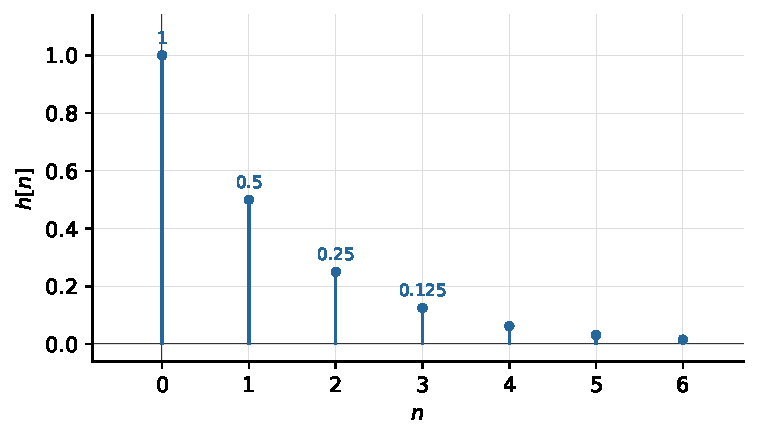
\includegraphics[width=0.78\textwidth]{10-z-transform/examples/recursive-answer.pdf}
    \caption{例题 \ref{ex:dt-recursive-impulse} 的单位脉冲响应。$h[0]=1$，每个样值都是前一个的一半，序列向右侧无限延伸。}
    \label{fig:ex-dt-recursive-answer}
  \end{figure}

  稳定性用绝对值求和判断。等比级数公比为 $\frac12$，绝对值小于 $1$，
  \[
    \sum_{n=-\infty}^{\infty}|h[n]|=\sum_{n=0}^{\infty}\left(\frac12\right)^n=2<\infty,
  \]
  故系统 BIBO 稳定。

  按定义求 $h[n]$ 的 Z 变换，
  \[
    H(z)=\sum_{n=-\infty}^{\infty}h[n]z^{-n}
    =\sum_{n=0}^{\infty}\left(\frac12z^{-1}\right)^n
    =\frac1{1-\frac12z^{-1}}.
  \]
  等比级数在 $\left|\frac12z^{-1}\right|<1$ 时收敛，即 $|z|>\frac12$。极点 $z=\frac12$ 落在单位圆内，单位圆 $|z|=1$ 位于收敛域中，与稳定性结论一致。
\end{solution}

\begin{technique}
  递推求 $h[n]$ 时写清三件事：输入的脉冲位置、每一步用到的上一个输出、初始静止给出的负下标零值。算出前四个样值后先看比值是否恒定，恒定即为等比，公比恰好是方程中 $y[n-1]$ 的系数。最后用绝对值求和判稳定，并核对收敛域是否包含单位圆。
\end{technique}

\section{初始静止与输入超前项}
\label{sec:dt-initial-rest-example}

\begin{workedexample}[输入含超前冲激时的递推]
  \label{ex:dt-recursive-difference}
  因果、初始静止的离散 LTI 系统满足
  \[
    y[n]-\frac12y[n-1]=x[n],
  \]
  输入为
  \[
    x[n]=-2\impulse[n+1]+\stepfun[n],
  \]
  题图见\cref{fig:ex-dt-difference-given}。求输出 $y[n]$。
  \begin{figure}[H]
    \centering
    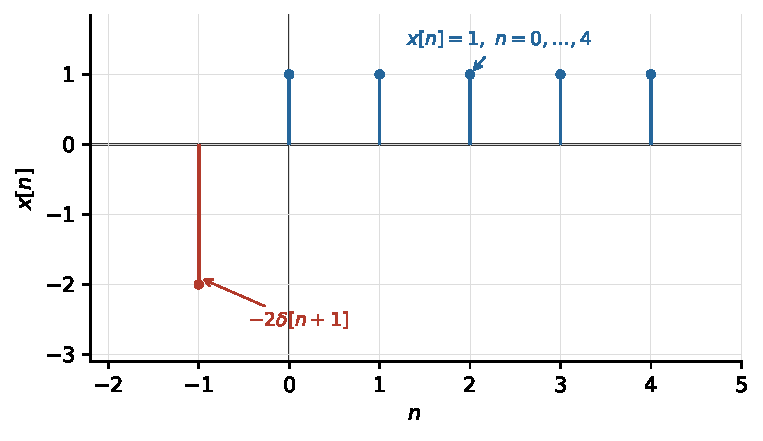
\includegraphics[width=0.78\textwidth]{10-z-transform/examples/first-order-difference-given.pdf}
    \caption{例题 \ref{ex:dt-recursive-difference} 的输入序列：$n=-1$ 处有一个权为 $-2$ 的冲激，$n=0$ 至 $4$ 取值为 $1$。}
    \label{fig:ex-dt-difference-given}
  \end{figure}
\end{workedexample}

\begin{solution}
  输入在 $n=-1$ 处已经非零，按初始静止只能写出 $y[n]=0$（$n<-1$），不能直接取 $y[-1]=0$。递推式仍为
  \[
    y[n]=x[n]+\frac12y[n-1],
  \]
  从 $n=-1$ 起步：
  \begin{align*}
    y[-1]&=x[-1]+\frac12y[-2]=-2+0=-2,\\
    y[0]&=x[0]+\frac12y[-1]=1-1=0,\\
    y[1]&=x[1]+\frac12y[0]=1+0=1,\\
    y[2]&=x[2]+\frac12y[1]=1+\frac12=\frac32,\\
    y[3]&=x[3]+\frac12y[2]=1+\frac34=\frac74,\\
    y[4]&=x[4]+\frac12y[3]=1+\frac78=\frac{15}8.
  \end{align*}
  从 $n=1$ 起输入恒为 $1$，递推规律稳定下来。记 $y[n]=\frac12y[n-1]+1$，两边减去稳态值 $2$：
  \[
    y[n]-2=\frac12\bigl(y[n-1]-2\bigr),
  \]
  故 $y[n]=2+\left(\frac12\right)^n\bigl(y[0]-2\bigr)$。代入 $y[0]=0$，得 $y[n]=2-2\left(\frac12\right)^n=2-2^{1-n}$（$n\geq0$）。
  核对 $n=1,2,3$：$2-1=1$，$2-\frac12=\frac32$，$2-\frac14=\frac74$，与逐项计算一致。合并两段，
  \[
    \boxed{
    y[n]=
    \begin{cases}
      -2,&n=-1,\\
      2-2^{1-n},&n\geq0,\\
      0,&n<-1.
    \end{cases}}
  \]
  输出从 $n=0$ 起由 $0$ 单调上升到稳态值 $2$，见\cref{fig:ex-dt-difference-answer}。
  \begin{figure}[H]
    \centering
    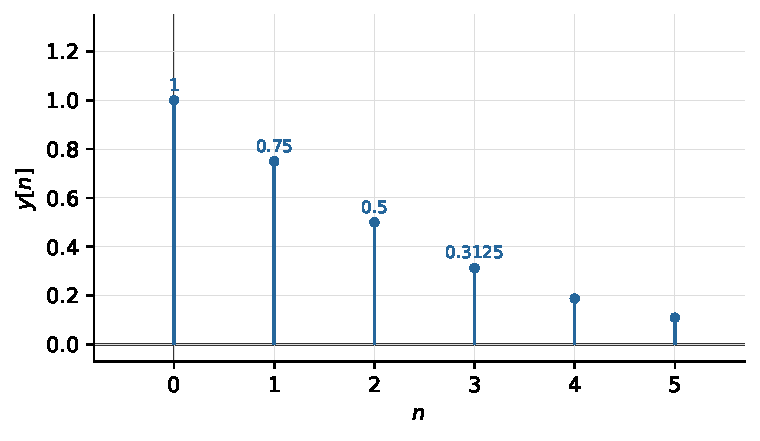
\includegraphics[width=0.78\textwidth]{10-z-transform/examples/first-order-difference-answer.pdf}
    \caption{例题 \ref{ex:dt-recursive-difference} 的输出序列：$n=-1$ 处的负冲激使 $y[0]$ 被抬回零，此后逐项趋近稳态值 $2$。}
    \label{fig:ex-dt-difference-answer}
  \end{figure}
\end{solution}

\begin{technique}
  输入含 $\impulse[n+n_0]$ 时，先按初始静止把零区间确定下来，再从最早的非零下标开始递推。逐项算到输入转为常值后，可用稳态值移位：把递推式两边减去稳态值，使余量成为等比数列，一次求出闭式。首项必须与逐项计算的最早几个值对上，否则差值公式用错了起点。
\end{technique}

\section{含输入延时项的差分方程}
\label{sec:dt-input-delay-example}

\begin{workedexample}[含输入延时项的方程]
  \label{ex:dt-input-delay}
  因果、初始静止的离散 LTI 系统满足
  \[
    y[n]-\frac16y[n-1]-\frac16y[n-2]=2x[n]+x[n-1].
  \]
  求单位脉冲响应 $h[n]$，判断系统的稳定性，再求 $x[n]=\left(\frac12\right)^n\stepfun[n]$ 时的零状态响应。
\end{workedexample}

\begin{solution}
  先取 $x[n]=\impulse[n]$。右端只在 $n=0,1$ 处提供数值：
  \[
    2\impulse[n]+\impulse[n-1]=
    \begin{cases}
      2,&n=0,\\
      1,&n=1,\\
      0,&\text{其他}.
    \end{cases}
  \]
  递推式
  \[
    y[n]=\frac16y[n-1]+\frac16y[n-2]+2\impulse[n]+\impulse[n-1]
  \]
  从 $n=0$ 起逐项计算，负下标处由初始静止取零：
  \begin{align*}
    h[0]&=\frac16h[-1]+\frac16h[-2]+2=2,\\
    h[1]&=\frac16h[0]+\frac16h[-1]+1=\frac13+1=\frac43,\\
    h[2]&=\frac16h[1]+\frac16h[0]=\frac29+\frac13=\frac59,\\
    h[3]&=\frac16h[2]+\frac16h[1]=\frac5{54}+\frac29=\frac{17}{54},\\
    h[4]&=\frac16h[3]+\frac16h[2]=\frac{17}{324}+\frac5{54}=\frac{47}{324}.
  \end{align*}
  前两项受输入直接激励，从 $n=2$ 起输入为零，递推依特征根展开。解特征方程
  \[
    \lambda^2-\frac16\lambda-\frac16=0
    \quad\Longleftrightarrow\quad
    \bigl(\lambda-\tfrac12\bigr)\bigl(\lambda+\tfrac13\bigr)=0,
  \]
  两个特征根为 $\frac12$ 与 $-\frac13$，$n\geq0$ 上的脉冲响应应取
  \[
    h[n]=A\left(\frac12\right)^n+B\left(-\frac13\right)^n.
  \]
  用前两个样值定系数：
  \[
    A+B=2,\qquad \frac A2-\frac B3=\frac43.
  \]
  第二式两端乘 $6$ 得 $3A-2B=8$，与第一式联立解得 $A=\frac{12}5$、$B=-\frac25$。因此
  \[
    \boxed{h[n]=\frac{12}5\left(\frac12\right)^n\stepfun[n]
                  -\frac25\left(-\frac13\right)^n\stepfun[n]}.
  \]
  两个参数的绝对值都小于 $1$，故 $\sum_{n=-\infty}^{\infty}|h[n]|<\infty$，系统 BIBO 稳定。

  求给定输入下的零状态响应时，逐点做卷积和代价较高，改用 Z 变换。对原方程逐项变换，
  \[
    \left(1-\frac16z^{-1}-\frac16z^{-2}\right)Y(z)
    =\left(2+z^{-1}\right)X(z),
  \]
  故
  \[
    H(z)=\frac{2+z^{-1}}{\left(1-\frac12z^{-1}\right)\left(1+\frac13z^{-1}\right)}.
  \]
  输入 $\left(\frac12\right)^n\stepfun[n]$ 的变换为 $X(z)=1/\left(1-\frac12z^{-1}\right)$，它使 $H(z)$ 中第一个因子重复：
  \[
    Y(z)=\frac{2+z^{-1}}
      {\left(1-\frac12z^{-1}\right)^2\left(1+\frac13z^{-1}\right)}.
  \]
  设
  \[
    Y(z)=\frac{P}{1-\frac12z^{-1}}
      +\frac{Q}{\left(1-\frac12z^{-1}\right)^2}
      +\frac{R}{1+\frac13z^{-1}}.
  \]
  记 $q=z^{-1}$，清除分母得到多项式恒等式
  \[
    2+q=P\left(1-\tfrac12q\right)\left(1+\tfrac13q\right)
        +Q\left(1+\tfrac13q\right)
        +R\left(1-\tfrac12q\right)^2.
  \]
  依次代入使各因子为零的 $q$：
  \begin{align*}
    q&=2:\quad 4=Q\left(1+\tfrac23\right)\Rightarrow Q=\frac{12}5,\\
    q&=-3:\quad -1=R\left(1+\tfrac32\right)^2\Rightarrow R=-\frac4{25},\\
    q&=0:\quad 2=P+Q+R\Rightarrow P=2-\frac{12}5+\frac4{25}=-\frac6{25}.
  \end{align*}
  反演时用两个标准变换对
  \[
    \frac1{1-\frac12z^{-1}}\longleftrightarrow\left(\frac12\right)^n\stepfun[n],
    \qquad
    \frac1{\left(1-\frac12z^{-1}\right)^2}
    \longleftrightarrow(n+1)\left(\frac12\right)^n\stepfun[n],
  \]
  得到
  \[
    y[n]=\left[\frac{12}5(n+1)-\frac6{25}\right]\left(\frac12\right)^n\stepfun[n]
      -\frac4{25}\left(-\frac13\right)^n\stepfun[n].
  \]
  把方括号内合并，
  \[
    \boxed{
    y[n]=\left[\frac{60n+54}{25}\left(\frac12\right)^n
      -\frac4{25}\left(-\frac13\right)^n\right]\stepfun[n]}.
  \]

  用原递推式核对。输入满足 $x[0]=1$，$x[1]=\frac12$，$x[2]=\frac14$，负下标为零：
  \begin{align*}
    y[0]&=\frac16y[-1]+\frac16y[-2]+2x[0]+x[-1]=2,\\
    y[1]&=\frac16y[0]+\frac16y[-1]+2x[1]+x[0]
        =\frac13+0+1+1=\frac73,\\
    y[2]&=\frac16y[1]+\frac16y[0]+2x[2]+x[1]
        =\frac7{18}+\frac13+\frac12+\frac12=\frac{31}{18}.
  \end{align*}
  把 $n=0,1,2$ 代入反演结果：
  \[
    y[0]=\frac{54}{25}-\frac4{25}=2,
  \]
  \[
    y[1]=\frac{114}{25}\cdot\frac12+\frac4{75}
        =\frac{57}{25}+\frac4{75}
        =\frac{171+4}{75}=\frac{175}{75}=\frac73,
  \]
  \[
    y[2]=\frac{174}{25}\cdot\frac14-\frac4{225}
        =\frac{87}{50}-\frac4{225}
        =\frac{783-8}{450}=\frac{775}{450}=\frac{31}{18}.
  \]
  三处取值都与递推结果一致。负下标处取零，与初始静止条件吻合。
\end{solution}

\begin{technique}
  右端含 $x[n-1]$ 等延时项时，脉冲响应开头几个样值由输入直接决定，之后才依特征根展开，定系数要用最早的两个非零样值。输入使某个一次因子重复时，部分分式必须同时保留二次项与一次项。系数在清除分母后的多项式恒等式中求出，三处 $q$ 的取值分别给出 $Q$、$R$ 与 $P$。反演后务必回到原递推式核对 $n=0,1,2$，逐个样值对照能查出系数或输入取值上的错误。
\end{technique}

\section{由单位延时器构成的方框图}
\label{sec:dt-block-diagram}

离散时间的方框图用三种基本单元：加法器、数乘器与单位延时器。单位延时器把当前的输入存下来，下一个时刻输出 $x[n-1]$，它承担的记忆作用与连续时间里的积分器相当。

一阶差分方程
\[
  y[n]+ay[n-1]=bx[n]
\]
先解出 $y[n]$，
\begin{equation}
  y[n]=-ay[n-1]+bx[n],
  \label{eq:dt-block-diagram-form}
\end{equation}
右端需要 $x[n]$ 与 $y[n-1]$ 各乘一个系数后相加。把 $y[n]$ 经单位延时器得到 $y[n-1]$，数乘 $-a$ 后与 $bx[n]$ 相加，即得 $y[n]$；计算结果又送回延时器，构成反馈，这正是\cref{eq:dt-recursive-form} 递推性质的图形表示。

\begin{remark}[两种方框图的对应]
  连续时间用积分器，离散时间用单位延时器，两者的差别只在存储量的含义：积分器存的是累积面积，延时器存的是上一个样值。初始静止在连续时间对应积分器初值为零，在离散时间对应\red{延时器初值为零}，也就是 $y[n]=0$（$n<n_0$）。方框图中每个延时器都需要初值，这也是 $N$ 阶方程需要 $N$ 个辅助条件的原因。
\end{remark}

\begin{remark}[与变换域解法的衔接]
  初始静止下对\cref{eq:dt-lccde} 两端作 Z 变换，延时 $k$ 变成乘 $z^{-k}$，差分方程化为关于 $z$ 的代数方程。本节两道递推例题都能用这条路线重算：分母的因式分解给出特征根，$H(z)$ 的分母因式与 $h[n]$ 的指数项一一对应，部分分式系数由初始静止条件确定。高阶方程用变换域求解的代数步骤少得多，这是后续各节展开 Z 变换方法的主要动因。
\end{remark}
